\section{Approaches}

Before starting the actual implementation process, we first thought about different
ways in which the Lanczos algorithm could be realized in the Apache Flink system. We
identified three different approaches that we could take. One of them would be to
leverage Flink's delta iteration construction, another one would be to make use of
Mahout's implementation of the Lanczos algorithm for the Hadoop framework. The third
possibility we found is to still implement the actual algorithm manually in Flink, but
without using delta iterations to model the algorithm's iterative nature.


% Approach: Delta Iterations
% ==========================

\subsection{Using Flink Delta Iterations}
\label{ssec:delta_iterations}

While planning the implementation part of our project, we consulted both the official
Flink 0.8 documentation [1] as well as the Flink community directly (mainly through
the \#flink IRC channel in the Freenode IRC network) in order to find reasonable
approaches for our intent. The first and most obvious approach both of these sources 
pointed to was to take advantage of Flink's delta iteration capabilities. But what
exactly are delta iterations, how do they compare to standard Flink iterations and why 
would we choose the former over the latter?

% General Description of Flink's Iterations
% -----------------------------------------

Flink provides an iteration operator specifically for the purpose of implementing
iterative algorithms, as these kinds of algorithms occur in many domains of data
analysis and as the general interest in running them on huge data sets is increasing.
The mere existence of this special kind of operator (and the fact that we were explicitly
pointed to it by the Flink community) led us to the conclusion that this must be the
idiomatic way of implementing the Lanczos algorithm in Flink. Two variants of the
iteration operator are provided by Flink: \textbf{Iterate} (we will also call this the
standard iteration) and \textbf{Delta Iterate}. The general idea of both of these operators
is that the programmer defines a step function that will be invoked repeatedly on the
current state of the data until a specified termination condition is reached. [1]

% Iterate Operator
% ----------------

% TODO: Are we allowed to use images from the Flink documentation?
\begin{figure}[h]
	\centering
	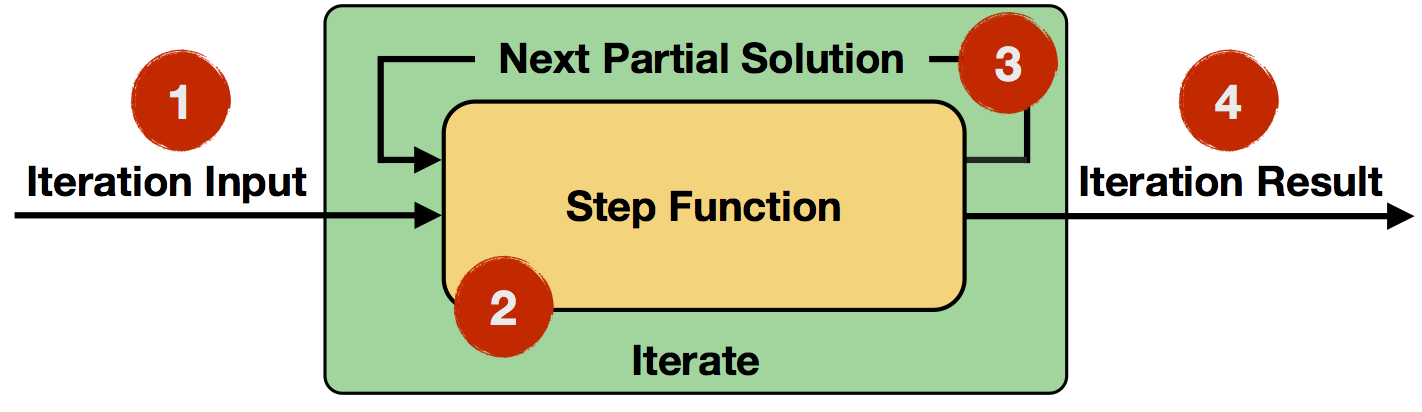
\includegraphics[width=0.8\textwidth]{images/iterations_iterate_operator}
	\caption{Graphical representation of the Iterate operator's data flow (source: 
	The Apache Software Foundation [1])}
	\label{fig:iterate_operator}
\end{figure}

Intended to be used for rather simple forms of iteration, the step function (2) of the 
\textbf{Iterate} operator, pictured in figure \ref{fig:iterate_operator}, always takes the 
entire input and computes the next partial solution from that (3). While the first step's input 
is the initial data set specified by the programmer (1), every step that follows consumes the 
partial solution produced by the preceding step. The Iterate operator's final result is simply 
the partial solution produced by the very last step (4). [1]

% Delta Iterate Operator
% ----------------------

\begin{figure}[h]
	\centering
	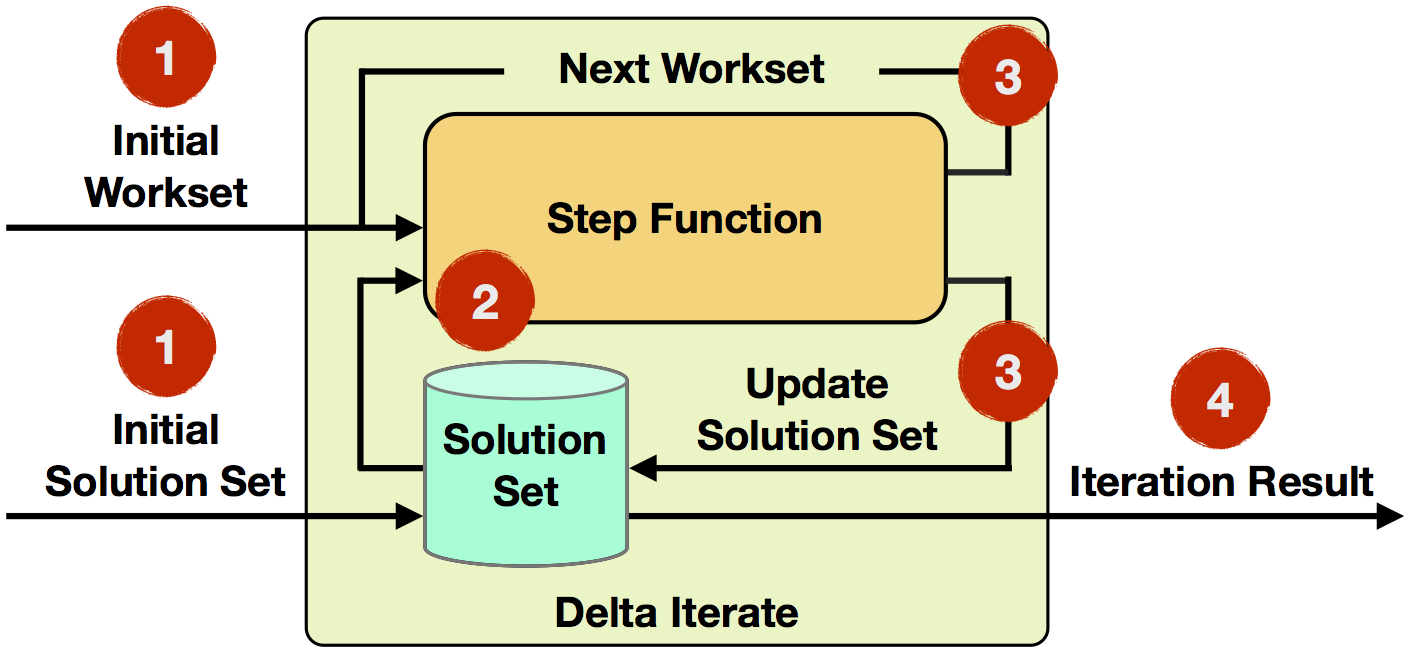
\includegraphics[width=0.8\textwidth]{images/iterations_delta_iterate_operator}
	\caption{Graphical representation of the Delta Iterate operator's data flow (source: 
	The Apache Software Foundation [1])}
	\label{fig:delta_iterate_operator}
\end{figure}

On the other hand, Flink's \textbf{Delta Iterate} operator, visualized in figure 
\ref{fig:delta_iterate_operator}, is specifically designed for implementing incremental
iterations that only modify small parts of the final result in every iteration step and that 
thus continually evolve the final result rather than fully recomputing it in every step.
Compared to standard iterations, delta iterations bring a performance benefit to the table,
as each of their steps only operates on a small subset of the data. Flink's delta iterations
use a work set and a solution set. While every work set instance only exists for one single
iteration, there is only one instance of the solution set whose state is persisted throughout 
all the iteration steps. The initial values of these two sets (1) are specified by the 
programmer. In every iteration, the step function (2) takes the current work set and the current
state of the solution set as its input and produces a new work set while also (optionally)
updating the contents of the solution set (3). The final result of a delta iteration is
contained in the solution set after the last iteration step has terminated (4). [1]

% Conclusion: Why DELTA iterations for Lanczos?
% ---------------------------------------------

As described in section \ref{sec:lanczos}, every iteration of the Lanczos algorithm only needs
(parts of) the result of the preceding iteration. Also, during every iteration, the final result
is only appended by small parts and none of its existing parts are modified in any way. This
scheme seems to perfectly match the way Flink's delta iterations work, which is why we decided
that delta iterations are more appropriate than standard iterations for implementing the Lanczos
algorithm in Flink.


% Approach: Using Mahout's LanczosSolver
% ======================================

\subsection{Using Mahout's Implementation of the Lanczos Algorithm}

During the research phase of our project, we studied (amongst others) the documentation [2]
and the source code [3] of the Apache Mahout machine learning library. It quickly came to our
attention that Mahout contains a full SVD implementation using the Lanczos algorithm. The
algorithm itself is implemented in the \texttt{LanczosSolver} class in Mahout's \texttt{math}
package. At first we only studied this implementation in order to learn more about the way the
algorithm works as well as for inspiration purposes. Eventually we started to consider reusing
this existing implementation to run the Lanczos algorithm in Flink.

% Brief description of Mahout approach
% ------------------------------------

Directly using Mahout's \texttt{LanczosSolver} for our project would include implementing all
the interfaces and possibly extending most of the classes that are used within the
\texttt{LanczosSolver} class and then running it on those implementations of ours. That way, we
wouldn't actually implement the algorithm itself for Flink. Instead, we would implement sort of
an Add-On that would allow the \texttt{LanczosSolver} to be run on a Flink cluster. The benefits
of that kind of code reuse include a relatively high confidence in the correctness of the
algorithm's actual implementation. Also, the efforts that would be saved by not implementing the
whole algorithm ourselves could potentially be spent on getting things up and running more
quickly and on improving other parts of the system.


% Loop-Based Approach
% ===================

\subsection{Loop-Based implementation}

The approach that actually came to our minds first was to implement the Lanczos algorithm in a
loop-based fashion, modeling data flow effectively the same way you would model it when
implementing a non-iterative algorithm in Flink. As we had previously never been exposed to
Flink's delta iterations in practice, modeling data flow the way we were used to from previous
exercises was the most intuitive approach for us.

In this approach, the algorithm's iterative nature is not modeled by leveraging Flink's special
iteration constructs, but by using ordinary Java loops instead. Rather than letting Flink's
internals deal with work set and solution set (see \ref{ssec:delta_iterations}), we figured we
could manually manage the various data sets needed for the final results, for intermediate
results that are needed in the next iteration as well as for temporary data that is only needed
'locally' within a single iteration.

% Brief explanation of Flink execution flow
% -----------------------------------------

In order to understand the potential downsides of this approach, a basic understanding of how
Flink programs are executed is necessary. When running a Flink program, that program is not
executed directly\footnote{Of course, the bytecode that results from compiling said Flink
program is executed directly, however Flink doesn't execute the data flow specified by the
program immediately.}. Instead, Flink compiles the program to an execution plan, which is then
executed [4]. Before executing said plan, which is basically a graph representing the program's
whole data flow, Flink tries to optimize it for speed and/or storage performance.

% Impact of Flink execution flow on loop-based approach
% -----------------------------------------------------

Now the main potential problem with the loop-based approach is that Flink doesn't really know
about the iterative nature of the implemented algorithm and that the program can thus not be
optimized completely by Flink. Taking that into consideration, we expected this approach (while
certainly being possible) to implicate performance loss of some kind compared to the delta
iteration approach described in section \ref{ssec:delta_iterations}.

